\chapter{Matrices}

\index{matriz}

Una \key{matriz} es un concepto matemático que corresponde a un arreglo
bidimensional en la programación. Por ejemplo,
\[
    A =
    \begin{bmatrix}
        6 & 13 & 7 & 4  \\
        7 & 0  & 8 & 2  \\
        9 & 5  & 4 & 18 \\
    \end{bmatrix}
\]
es una matriz de tamaño $3 \times 4$, o sea que tiene 3 filas y 4 columnas.
La notación $[i,j]$ se refiere al elemento en fila $i$ y columna $j$ en una
matriz. Por ejemplo, en la matriz de arriba, $A[2,3]=8$ y $A[3,1]=9$.

\index{vector}
Un caso especial de una matriz es el \key{vector}, una matriz
unidimensional de tamaño $n \times 1$. Por ejemplo,
\[
    V =
    \begin{bmatrix}
        4 \\
        7 \\
        5 \\
    \end{bmatrix}
\]
es un vector que contiene tres elementos.

\index{transpuesta}

La matriz \key{transpuesta} $A^T$ de una matriz $A$ es obtenida cuando
las filas y columnas de $A$ son intercambiadas, o sea, $A^T[i,j]=A[j,i]$:
\[
    A^T =
    \begin{bmatrix}
        6  & 7 & 9  \\
        13 & 0 & 5  \\
        7  & 8 & 4  \\
        4  & 2 & 18 \\
    \end{bmatrix}
\]

\index{matriz!cuadrada}
Una matriz se denomina \key{matriz cuadrada} si tiene el mismo número de filas
que de columnas. Por ejemplo, la siguiente matriz es cuadrada:
\[
    S =
    \begin{bmatrix}
        3 & 12 & 4  \\
        5 & 9  & 15 \\
        0 & 2  & 4  \\
    \end{bmatrix}
\]

\section{Operaciones}

La suma $A+B$ de las matrices $A$ y $B$ está definida si las matrices son del
mismo tamaño. El resultado es una matriz donde cada elemento es la suma de los
elementos correspondientes en $A$ y $B$.

Por ejemplo,
\[
    \begin{bmatrix}
        6 & 1 & 4 \\
        3 & 9 & 2 \\
    \end{bmatrix}
    +
    \begin{bmatrix}
        4 & 9 & 3 \\
        8 & 1 & 3 \\
    \end{bmatrix}
    =
    \begin{bmatrix}
        6+4 & 1+9 & 4+3 \\
        3+8 & 9+1 & 2+3 \\
    \end{bmatrix}
    =
    \begin{bmatrix}
        10 & 10 & 7 \\
        11 & 10 & 5 \\
    \end{bmatrix}.
\]

Multiplicar una matriz $A$ por un valor $x$ significa que cada elemento de $A$
es multiplicado por $x$. Por ejemplo,
\[
    2 \cdot \begin{bmatrix}
        6 & 1 & 4 \\
        3 & 9 & 2 \\
    \end{bmatrix}
    =
    \begin{bmatrix}
        2 \cdot 6 & 2\cdot1 & 2\cdot4 \\
        2\cdot3   & 2\cdot9 & 2\cdot2 \\
    \end{bmatrix}
    =
    \begin{bmatrix}
        12 & 2  & 8 \\
        6  & 18 & 4 \\
    \end{bmatrix}.
\]

\subsubsection{Multiplicación de matrices}

\index{multiplicación de matrices}

El producto $AB$ de las matrices $A$ y $B$ está definido si $A$ es de tamaño
$a \times n$ y $B$ es de tamaño $n \times b$, o sea, el ancho de $A$ equivale
a la altura de $B$. El resultado es una matriz de tamaño $a \times b$ cuyos
elementos son calculados usando la fórmula
\[
    AB[i,j] = \sum_{k=1}^n A[i,k] \cdot B[k,j].
\]

La idea es que cada elemento de $AB$ es una suma de productos de elementos de
$A$ y $B$, como vemos en la siguiente imagen:

\begin{center}
    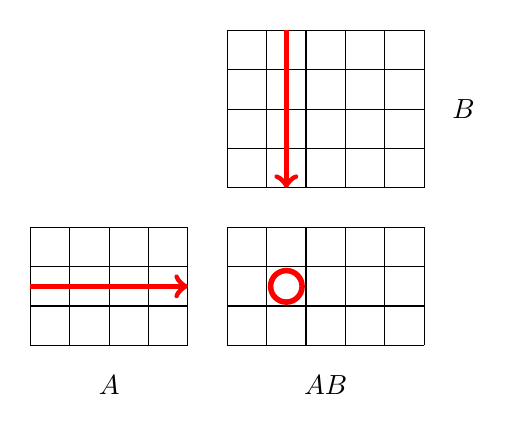
\begin{tikzpicture}[scale=0.5]
        \draw (0,0) grid (4,3);
        \draw (5,0) grid (10,3);
        \draw (5,4) grid (10,8);

        \node at (2,-1) {$A$};
        \node at (7.5,-1) {$AB$};
        \node at (11,6) {$B$};

        \draw[thick,->,red,line width=2pt] (0,1.5) -- (4,1.5);
        \draw[thick,->,red,line width=2pt] (6.5,8) -- (6.5,4);
        \draw[thick,red,line width=2pt] (6.5,1.5) circle (0.4);
    \end{tikzpicture}
\end{center}

Por ejemplo,

\[
    \begin{bmatrix}
        1 & 4 \\
        3 & 9 \\
        8 & 6 \\
    \end{bmatrix}
    \cdot
    \begin{bmatrix}
        1 & 6 \\
        2 & 9 \\
    \end{bmatrix}
    =
    \begin{bmatrix}
        1 \cdot 1 + 4 \cdot 2 & 1 \cdot 6 + 4 \cdot 9 \\
        3 \cdot 1 + 9 \cdot 2 & 3 \cdot 6 + 9 \cdot 9 \\
        8 \cdot 1 + 6 \cdot 2 & 8 \cdot 6 + 6 \cdot 9 \\
    \end{bmatrix}
    =
    \begin{bmatrix}
        9  & 42  \\
        21 & 99  \\
        20 & 102 \\
    \end{bmatrix}.
\]

La multiplicación de matrices es asociativa, así que $A(BC)=(AB)C$, pero
no es conmutativa, por lo que $AB = BA$ no necesariamente se cumple.

\index{matriz!identidad}

Una \key{matriz identidad} es una matriz cuadrada en donde cada elemento en la
diagonal es 1 y todos los otros elementos son 0. Por ejemplo, la siguiente
matriz es la matriz de identidad $3 \times 3$:
\[
    I = \begin{bmatrix}
        1 & 0 & 0 \\
        0 & 1 & 0 \\
        0 & 0 & 1 \\
    \end{bmatrix}
\]

Multiplicar una matriz por una matriz identidad no la modifica. Por ejemplo,
\[
    \begin{bmatrix}
        1 & 0 & 0 \\
        0 & 1 & 0 \\
        0 & 0 & 1 \\
    \end{bmatrix}
    \cdot
    \begin{bmatrix}
        1 & 4 \\
        3 & 9 \\
        8 & 6 \\
    \end{bmatrix}
    =
    \begin{bmatrix}
        1 & 4 \\
        3 & 9 \\
        8 & 6 \\
    \end{bmatrix} \hspace{10px} \textrm{y} \hspace{10px}
    \begin{bmatrix}
        1 & 4 \\
        3 & 9 \\
        8 & 6 \\
    \end{bmatrix}
    \cdot
    \begin{bmatrix}
        1 & 0 \\
        0 & 1 \\
    \end{bmatrix}
    =
    \begin{bmatrix}
        1 & 4 \\
        3 & 9 \\
        8 & 6 \\
    \end{bmatrix}.
\]

Usando un sencillo algoritmo, podemos calcular el producto de dos matrices
con tamaño $n \times n$ en tiempo $O(n^3)$. También existen algoritmos más
eficientes para la multiplicación de matrices,\footnote{El primer algoritmo
    tal fue el algoritmo de Strassen, publicado en 1969\cite{str69}, cuya
    complejidad temporal es $O(n^{2,80735})$; el mejor algoritmo conocido
    actualmente \cite{gal14} funciona en $O(n^{2,37286})$.} pero
mayormente son de interés teórico y son innecesarios en la programación
competitiva.

\subsubsection{Exponenciación de matrices}

\index{exponenciación de matrices}

La potencia $A^k$ de una matriz $A$ está definida si $A$ es una matriz
cuadrada. La definición se basa en la multiplicación de matrices:
\[ A^k = \underbrace{A \cdot A \cdot A \cdots A}_{\textrm{$k$ times}} \]
Por ejemplo,

\[
    \begin{bmatrix}
        2 & 5 \\
        1 & 4 \\
    \end{bmatrix}^3 =
    \begin{bmatrix}
        2 & 5 \\
        1 & 4 \\
    \end{bmatrix} \cdot
    \begin{bmatrix}
        2 & 5 \\
        1 & 4 \\
    \end{bmatrix} \cdot
    \begin{bmatrix}
        2 & 5 \\
        1 & 4 \\
    \end{bmatrix} =
    \begin{bmatrix}
        48 & 165 \\
        33 & 114 \\
    \end{bmatrix}.
\]
Adicionalmente, $A^0$ es una matriz identidad. Por ejemplo,
\[
    \begin{bmatrix}
        2 & 5 \\
        1 & 4 \\
    \end{bmatrix}^0 =
    \begin{bmatrix}
        1 & 0 \\
        0 & 1 \\
    \end{bmatrix}.
\]

La matriz $A^k$ puede calcularse eficientemente en  $O(n^3 \log k)$
utilizando el algoritmo descrito en el Capítulo 21.2. Por ejemplo,
\[
    \begin{bmatrix}
        2 & 5 \\
        1 & 4 \\
    \end{bmatrix}^8 =
    \begin{bmatrix}
        2 & 5 \\
        1 & 4 \\
    \end{bmatrix}^4 \cdot
    \begin{bmatrix}
        2 & 5 \\
        1 & 4 \\
    \end{bmatrix}^4.
\]

\subsubsection{Determinante}

\index{determinante}
\index{cofactor}

La \key{determinante} $\det(A)$ de una matriz $A$ está definida si $A$ es
una matriz cuadrada. Si $A$ tiene tamaño $1 \times 1$, entonces
$\det(A)=A[1,1]$. La determinante de una matriz más grande es calculada
recursivamente utilizando la fórmula
\[\det(A)=\sum_{j=1}^n A[1,j] C[1,j],\]
donde $C[i,j]$ es el \key{cofactor} de $A$ en $[i,j]$.
El cofactor es calculado usando la fórmula
\[C[i,j] = (-1)^{i+j} \det(M[i,j]),\]
donde $M[i,j]$ se obtiene quitando la fila $i$ y columna $j$ de $A$. Debido
al coeficiente $(-1)^{i+j}$ en el cofactor, las determinantes son
alternadamente positivas y negativas.
\[
    \det
    \begin{pmatrix}
        3 & 4 \\
        1 & 6 \\
    \end{pmatrix}
    = 3 \cdot 6 - 4 \cdot 1 = 14
\]
y
\[
    \det
    \begin{pmatrix}
        2 & 4 & 3 \\
        5 & 1 & 6 \\
        7 & 2 & 4 \\
    \end{pmatrix}
    =
    2 \cdot
    \det
    \begin{pmatrix}
        1 & 6 \\
        2 & 4 \\
    \end{pmatrix}
    -4 \cdot
    \det
    \begin{pmatrix}
        5 & 6 \\
        7 & 4 \\
    \end{pmatrix}
    +3 \cdot
    \det
    \begin{pmatrix}
        5 & 1 \\
        7 & 2 \\
    \end{pmatrix}
    = 81.
\]

\index{matriz!inversa}

La determinante de $A$ nos dice si existe una \key{matriz inversa} $A^{-1}$
tal que $A \cdot A^{-1} = I$, donde $I$ es una matriz identidad. Resulta que
$A^{-1}$ existe exactamente cuando $\det(A) \neq 0$, y puede ser calculado
utilizando la fórmula

\[A^{-1}[i,j] = \frac{C[j,i]}{det(A)}.\]

Por ejemplo,

\[
    \underbrace{
        \begin{bmatrix}
            2 & 4 & 3 \\
            5 & 1 & 6 \\
            7 & 2 & 4 \\
        \end{bmatrix}
    }_{A}
    \cdot
    \underbrace{
        \frac{1}{81}
        \begin{bmatrix}
            -8 & -10 & 21  \\
            22 & -13 & 3   \\
            3  & 24  & -18 \\
        \end{bmatrix}
    }_{A^{-1}}
    =
    \underbrace{
        \begin{bmatrix}
            1 & 0 & 0 \\
            0 & 1 & 0 \\
            0 & 0 & 1 \\
        \end{bmatrix}
    }_{I}.
\]

\section{Recurrencia lineal}

\index{recurrencia lineal}

Una \key{recurrencia lineal} es una función $f(n)$ cuyos valores iniciales son
$f(0),\ldots,\\f(k-1)$ y valores mayores son calculados recursivamente con la
fórmula \[f(n) = c_1 f(n-1) + c_2 f(n-2) + \ldots + c_k f (n-k),\]
donde $c_1,c_2,\ldots,c_k$ son coeficientes constantes.

Podemos emplear la programación dinámica para calcular cualquier valor de
$f(n)$ en $O(kn)$ calculando todos los valores de $f(0),f(1),\ldots,f(n)$
uno tras otro. Sin embargo, si $k$ es pequeña, es posible calcular $f(n)$
mucho más eficientemente en $O(k^3 \log n)$ utilizando operaciones de matrices.

\subsubsection{Números de Fibonacci}

\index{número de Fibonacci}

Un simple ejemplo de una recurrencia lineal es la siguiente función que define
los números de Fibonacci:
\[
    \begin{array}{lcl}
        f(0) & = & 0             \\
        f(1) & = & 1             \\
        f(n) & = & f(n-1)+f(n-2) \\
    \end{array}
\]
En este caso, $k=2$ y $c_1=c_2=1$.

Para calcular números de Fibonacci eficientemente, representamos la fórmula
de Fibonacci como una matriz cuadrada $X$ de tamaño $2 \times 2$, tal que:
\[ X \cdot
    \begin{bmatrix}
        f(i)   \\
        f(i+1) \\
    \end{bmatrix}
    =
    \begin{bmatrix}
        f(i+1) \\
        f(i+2) \\
    \end{bmatrix}
\]
Por lo tanto, los valores $f(i)$ y $f(i+1)$ son dados como ``entrada'' para
$X$,, y $X$ calcula los valores $f(i+1)$ y $f(i+2)$ a partir de ellos.
Resulta que una matriz tal es

\[ X =
    \begin{bmatrix}
        0 & 1 \\
        1 & 1 \\
    \end{bmatrix}.
\]
\noindent
Por ejemplo,
\[
    \begin{bmatrix}
        0 & 1 \\
        1 & 1 \\
    \end{bmatrix}
    \cdot
    \begin{bmatrix}
        f(5) \\
        f(6) \\
    \end{bmatrix}
    =
    \begin{bmatrix}
        0 & 1 \\
        1 & 1 \\
    \end{bmatrix}
    \cdot
    \begin{bmatrix}
        5 \\
        8 \\
    \end{bmatrix}
    =
    \begin{bmatrix}
        8  \\
        13 \\
    \end{bmatrix}
    =
    \begin{bmatrix}
        f(6) \\
        f(7) \\
    \end{bmatrix}.
\]
Por lo tanto, podemos calcular $f(n)$ usando la fórmula
\[
    \begin{bmatrix}
        f(n)   \\
        f(n+1) \\
    \end{bmatrix}
    =
    X^n \cdot
    \begin{bmatrix}
        f(0) \\
        f(1) \\
    \end{bmatrix}
    =
    \begin{bmatrix}
        0 & 1 \\
        1 & 1 \\
    \end{bmatrix}^n
    \cdot
    \begin{bmatrix}
        0 \\
        1 \\
    \end{bmatrix}.
\]
El valor de $X^n$ puede calcularse en $O(\log n)$, por lo que el valor de
$f(n)$ también puede calcularse en $O(\log n)$.

\subsubsection{Caso general}

Ahora veamos el caso general donde $f(n)$ es cualquier recurrencia lineal.
Nuevamente, nuestro objetivo es construir una matriz $X$ para la cual

\[ X \cdot
    \begin{bmatrix}
        f(i)     \\
        f(i+1)   \\
        \vdots   \\
        f(i+k-1) \\
    \end{bmatrix}
    =
    \begin{bmatrix}
        f(i+1) \\
        f(i+2) \\
        \vdots \\
        f(i+k) \\
    \end{bmatrix}.
\]
Una matriz tal es
\[
    X =
    \begin{bmatrix}
        0      & 1       & 0       & 0       & \cdots & 0      \\
        0      & 0       & 1       & 0       & \cdots & 0      \\
        0      & 0       & 0       & 1       & \cdots & 0      \\
        \vdots & \vdots  & \vdots  & \vdots  & \ddots & \vdots \\
        0      & 0       & 0       & 0       & \cdots & 1      \\
        c_k    & c_{k-1} & c_{k-2} & c_{k-3} & \cdots & c_1    \\
    \end{bmatrix}.
\]
En las primeras $k-1$ filas, cada elemento es 0 excepto uno, que es 1.
Estas filas reemplazan a $f(i)$ por $f(i+1)$, $f(i+1)$ con $f(i+2)$, y así
sucesivamente. La última fila contiene los coeficientes de la recurrencia
para calcular el nuevo valor de $f(i+k)$.

Ahora, $f(n)$ puede calcularse en $O(k^3 \log n)$ usando la fórmula
\[
    \begin{bmatrix}
        f(n)     \\
        f(n+1)   \\
        \vdots   \\
        f(n+k-1) \\
    \end{bmatrix}
    =
    X^n \cdot
    \begin{bmatrix}
        f(0)   \\
        f(1)   \\
        \vdots \\
        f(k-1) \\
    \end{bmatrix}.
\]

\section{Grafos y matrices}

\subsubsection{Contar caminos}

Las potencias de la matriz de adyacencia de un grafo tienen una interesante
propiedad. Cuando $V$ es la matriz de adyacencia de un grafo no ponderado,
la matriz $V^n$ contiene los números de caminos de $n$ aristas entre nodos del
grafo.

Por ejemplo, para el grafo
\begin{center}
    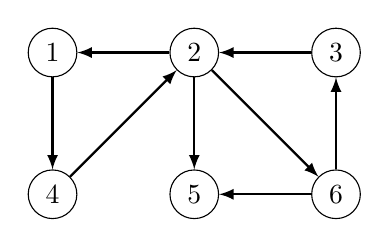
\begin{tikzpicture}[scale=0.9]
        \node[draw, circle] (1) at (1,3) {$1$};
        \node[draw, circle] (2) at (1,1) {$4$};
        \node[draw, circle] (3) at (3,3) {$2$};
        \node[draw, circle] (4) at (5,3) {$3$};
        \node[draw, circle] (5) at (3,1) {$5$};
        \node[draw, circle] (6) at (5,1) {$6$};

        \path[draw,thick,->,>=latex] (1) -- (2);
        \path[draw,thick,->,>=latex] (2) -- (3);
        \path[draw,thick,->,>=latex] (3) -- (1);
        \path[draw,thick,->,>=latex] (4) -- (3);
        \path[draw,thick,->,>=latex] (3) -- (5);
        \path[draw,thick,->,>=latex] (3) -- (6);
        \path[draw,thick,->,>=latex] (6) -- (4);
        \path[draw,thick,->,>=latex] (6) -- (5);
    \end{tikzpicture}
\end{center}
la matriz de adyacencia es
\[
    V= \begin{bmatrix}
        0 & 0 & 0 & 1 & 0 & 0 \\
        1 & 0 & 0 & 0 & 1 & 1 \\
        0 & 1 & 0 & 0 & 0 & 0 \\
        0 & 1 & 0 & 0 & 0 & 0 \\
        0 & 0 & 0 & 0 & 0 & 0 \\
        0 & 0 & 1 & 0 & 1 & 0 \\
    \end{bmatrix}.
\]
Ahora, por ejemplo, la matriz
\[
    V^4= \begin{bmatrix}
        0 & 0 & 1 & 1 & 1 & 0 \\
        2 & 0 & 0 & 0 & 2 & 2 \\
        0 & 2 & 0 & 0 & 0 & 0 \\
        0 & 2 & 0 & 0 & 0 & 0 \\
        0 & 0 & 0 & 0 & 0 & 0 \\
        0 & 0 & 1 & 1 & 1 & 0 \\
    \end{bmatrix}
\]
contiene los números de caminos de 4 aristas entre los nodos. Por ejemplo,
$V^4[2,5]=2$, porque existen dos nodos de 4 aristas entre el nodo 2 y 5:
$2 \rightarrow 1 \rightarrow 4 \rightarrow 2 \rightarrow 5$
y
$2 \rightarrow 6 \rightarrow 3 \rightarrow 2 \rightarrow 5$.

\subsubsection{Caminos mínimos}

Usando una idea similar en un grafo ponderado, podemos calcular para cada par
de nodos el mínimo camino de un camino entre ellos que contenga exactamente
$n$ aristas. Para calcular esto, debemos definir la multiplicación de matrices
de una forma nueva para, en vez de calcular los números de caminos, minizar
sus longitudes.

\pagebreak
Por ejemplo, considera el siguiente grafo:
\begin{center}
    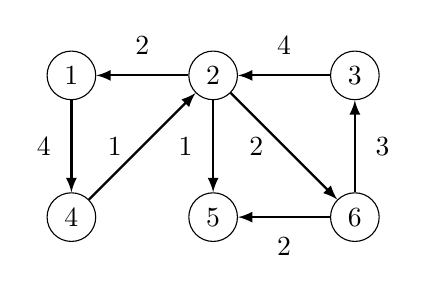
\begin{tikzpicture}[scale=0.9]
        \node[draw, circle] (1) at (1,3) {$1$};
        \node[draw, circle] (2) at (1,1) {$4$};
        \node[draw, circle] (3) at (3,3) {$2$};
        \node[draw, circle] (4) at (5,3) {$3$};
        \node[draw, circle] (5) at (3,1) {$5$};
        \node[draw, circle] (6) at (5,1) {$6$};

        \path[draw,thick,->,>=latex] (1) -- node[font=\small,label=left:4] {} (2);
        \path[draw,thick,->,>=latex] (2) -- node[font=\small,label=left:1] {} (3);
        \path[draw,thick,->,>=latex] (3) -- node[font=\small,label=north:2] {} (1);
        \path[draw,thick,->,>=latex] (4) -- node[font=\small,label=north:4] {} (3);
        \path[draw,thick,->,>=latex] (3) -- node[font=\small,label=left:1] {} (5);
        \path[draw,thick,->,>=latex] (3) -- node[font=\small,label=left:2] {} (6);
        \path[draw,thick,->,>=latex] (6) -- node[font=\small,label=right:3] {} (4);
        \path[draw,thick,->,>=latex] (6) -- node[font=\small,label=below:2] {} (5);
    \end{tikzpicture}
\end{center}

Consideremos una matriz de adyacencia donde $\infty$ significa que una arista
no existe, y otros valores corresponden a pesos de aristas. La matriz es
\[
    V= \begin{bmatrix}
        \infty & \infty & \infty & 4      & \infty & \infty \\
        2      & \infty & \infty & \infty & 1      & 2      \\
        \infty & 4      & \infty & \infty & \infty & \infty \\
        \infty & 1      & \infty & \infty & \infty & \infty \\
        \infty & \infty & \infty & \infty & \infty & \infty \\
        \infty & \infty & 3      & \infty & 2      & \infty \\
    \end{bmatrix}.
\]

En vez de la fórmula
\[
    AB[i,j] = \sum_{k=1}^n A[i,k] \cdot B[k,j]
\]
ahora utilizaremos la fórmula
\[
    AB[i,j] = \min_{k=1}^n A[i,k] + B[k,j]
\]
para multiplicación de matrices, así que calculamos un mínimo en vez de una
suma, y una suma de elementos en vez de un producto. Luego de esta
modificación, las potencias de una matriz corresponden a los caminos mínimos
en el grafo.

Por ejemplo, como
\[
    V^4= \begin{bmatrix}
        \infty & \infty & 10     & 11     & 9      & \infty \\
        9      & \infty & \infty & \infty & 8      & 9      \\
        \infty & 11     & \infty & \infty & \infty & \infty \\
        \infty & 8      & \infty & \infty & \infty & \infty \\
        \infty & \infty & \infty & \infty & \infty & \infty \\
        \infty & \infty & 12     & 13     & 11     & \infty \\
    \end{bmatrix},
\]
podemos concluir que la longitud mínima de un camino de 4 aristas entre
el nodo 2 y el nodo 5 es 8. Un camino tal es
$2 \rightarrow 1 \rightarrow 4 \rightarrow 2 \rightarrow 5$.

\pagebreak
\subsubsection{Teorema de Kirchhoff}

\index{teorema de Kirchhoff}
\index{árbol!de expansión!mínimo}

El \key{teorema de Kirchhoff} provee una manera de calcular el número de
árboles de expansión de un grafo como la determinante de una matriz especial.
Por ejemplo, el grafo
\begin{center}
    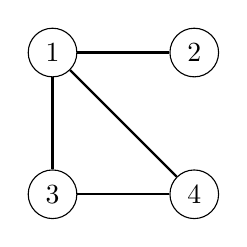
\begin{tikzpicture}[scale=0.9]
        \node[draw, circle] (1) at (1,3) {$1$};
        \node[draw, circle] (2) at (3,3) {$2$};
        \node[draw, circle] (3) at (1,1) {$3$};
        \node[draw, circle] (4) at (3,1) {$4$};

        \path[draw,thick,-] (1) -- (2);
        \path[draw,thick,-] (1) -- (3);
        \path[draw,thick,-] (3) -- (4);
        \path[draw,thick,-] (1) -- (4);
    \end{tikzpicture}
\end{center}
posee tres árboles de expansión:
\begin{center}
    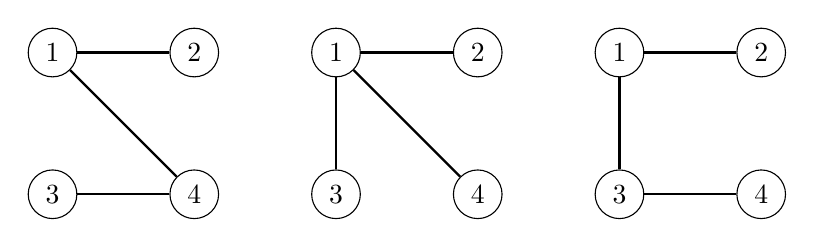
\begin{tikzpicture}[scale=0.9]
        \node[draw, circle] (1a) at (1,3) {$1$};
        \node[draw, circle] (2a) at (3,3) {$2$};
        \node[draw, circle] (3a) at (1,1) {$3$};
        \node[draw, circle] (4a) at (3,1) {$4$};

        \path[draw,thick,-] (1a) -- (2a);
        %\path[draw,thick,-] (1a) -- (3a);
        \path[draw,thick,-] (3a) -- (4a);
        \path[draw,thick,-] (1a) -- (4a);

        \node[draw, circle] (1b) at (1+4,3) {$1$};
        \node[draw, circle] (2b) at (3+4,3) {$2$};
        \node[draw, circle] (3b) at (1+4,1) {$3$};
        \node[draw, circle] (4b) at (3+4,1) {$4$};

        \path[draw,thick,-] (1b) -- (2b);
        \path[draw,thick,-] (1b) -- (3b);
        %\path[draw,thick,-] (3b) -- (4b);
        \path[draw,thick,-] (1b) -- (4b);

        \node[draw, circle] (1c) at (1+8,3) {$1$};
        \node[draw, circle] (2c) at (3+8,3) {$2$};
        \node[draw, circle] (3c) at (1+8,1) {$3$};
        \node[draw, circle] (4c) at (3+8,1) {$4$};

        \path[draw,thick,-] (1c) -- (2c);
        \path[draw,thick,-] (1c) -- (3c);
        \path[draw,thick,-] (3c) -- (4c);
        %\path[draw,thick,-] (1c) -- (4c);
    \end{tikzpicture}
\end{center}
\index{matriz!laplaciana}
Para calcular el número de árboles de expansión, construimos una
\key{matriz laplaciana} $L$, donde $L[i,i]$ es el grado del nodo $i$
y $L[i,j]=-1$ si hay una arista entre los nodos $i$ y $j$, y de lo
contrario $L[i,j]=0$. La matriz laplaciana para el grafo de arriba se ve así
\[
    L= \begin{bmatrix}
        3  & -1 & -1 & -1 \\
        -1 & 1  & 0  & 0  \\
        -1 & 0  & 2  & -1 \\
        -1 & 0  & -1 & 2  \\
    \end{bmatrix}
\]

Se puede demostrar que el número de árboles de expansión equivale a
la determinante de una matriz que es obtenida cuando quitamos cualquier
fila y cualquier columna de $L$. Por ejemplo, si quitamos la primera fila
y columna, el resultado es

\[ \det(
    \begin{bmatrix}
            1 & 0  & 0  \\
            0 & 2  & -1 \\
            0 & -1 & 2  \\
        \end{bmatrix}
    ) =3.\]
La determinante siempre es igual, independientemente de cuál fila y columna
quitemos de $L$.

Nota que la fórmula de Cayley (Capítulo 22.5) es un caso especial del teorema
de Kirchhoff, porque en un grafo completo de $n$ nodos

\[ \det(
    \begin{bmatrix}
            n-1    & -1     & \cdots & -1     \\
            -1     & n-1    & \cdots & -1     \\
            \vdots & \vdots & \ddots & \vdots \\
            -1     & -1     & \cdots & n-1    \\
        \end{bmatrix}
    ) =n^{n-2}.\]



